\newcommand{\norm}[1]{\Vert #1 \Vert}
\newcommand{\bigo}{\mathcal{O}}
\newcommand{\R}{\mathbb{R}}
\renewcommand{\Rn}[1]{\R^{#1}}
\newcommand{\Rmn}[2]{\R^{#1 \times #2}}

\section{Introduction}

\myframetop{
  \ctr{Julia Smooth Optimizers}

  \begin{minipage}{0.44\textwidth}
    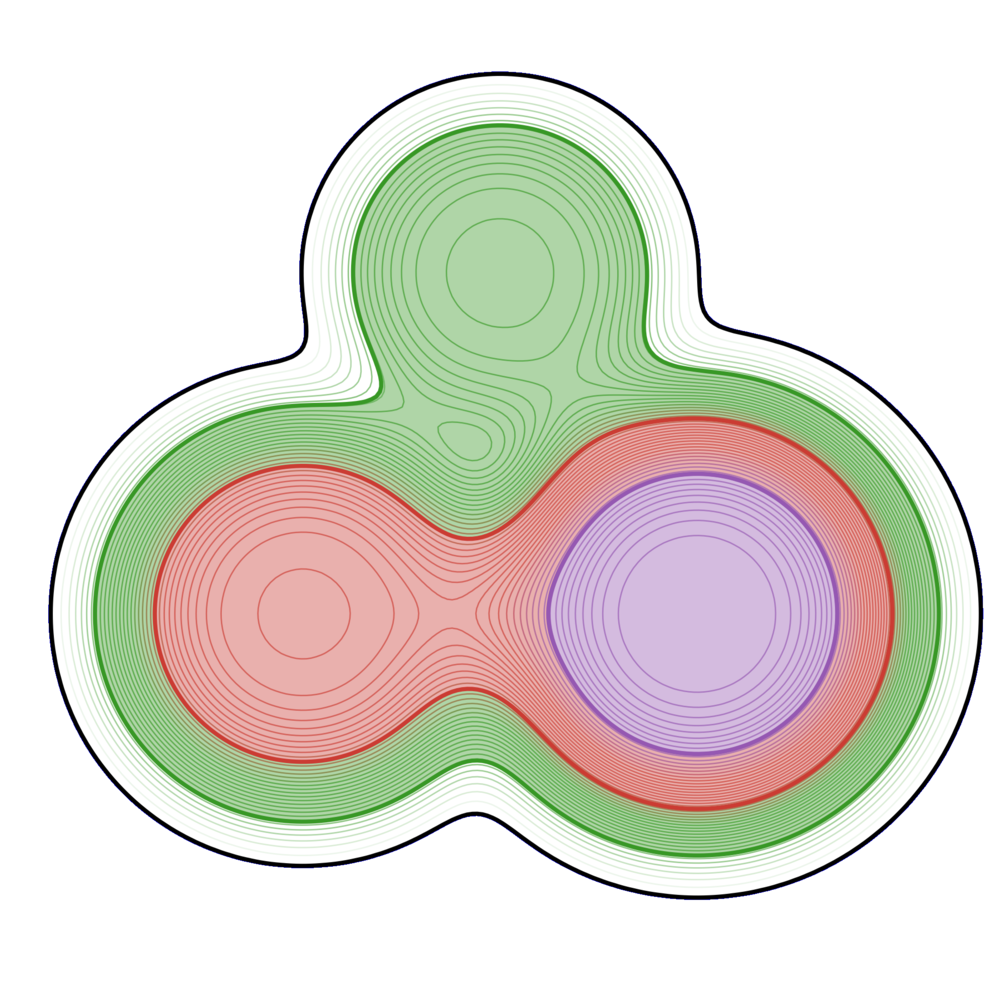
\includegraphics[height=0.75\textheight]{jsologo.png}
  \end{minipage}
  \begin{minipage}{0.55\textwidth}
    \begin{itemize}
      \item Linear Algebra and Optimization tools for developers/researchers/academics;
      \item Created from our demands;
      \item Integrates with MPB/JuMP (\cite{jump});
      \item We also develop solvers, focusing on large-scale;
      \item Similar work done previously in PythonOptimizers.
    \end{itemize}
  \end{minipage}
}

\myframetop{
  \ctr{Julia Smooth Optimizers}
  \begin{center}
    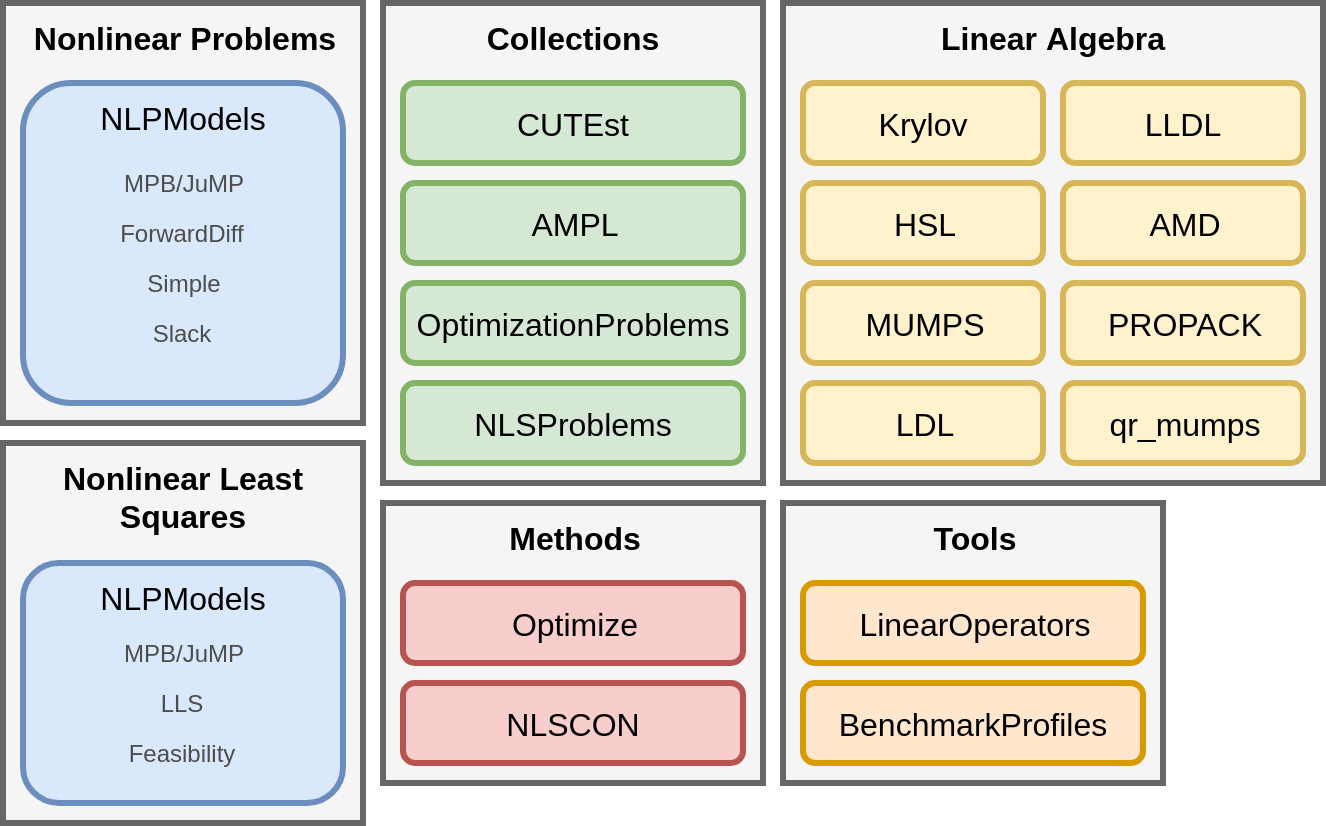
\includegraphics[height=0.75\textheight]{jsodesc.png}
  \end{center}
}

\section{NLPModels}

\begin{frame}[fragile,t]
  \ctr{NLPModels}

  \begin{itemize}
    \item Defines nonlinear programming models and unified API to access them;
    \item Some models provide sparse derivatives;
    \item Some models provide efficient matrix-free products (i.e. no explicit matrix
      used).
  \end{itemize}
\end{frame}

\begin{frame}[fragile,t]
  \ctr{NLPModels}
\begin{lstlisting}
  # Short
  adnlp = ADNLPModel(x -> (x[1] - 1)^2 + 100 * (x[2] - x[1]^2)^2, [-1.2; 1.0])

  # ROSENBR from the CUTEst list of problem
  ctnlp = CUTEstModel("ROSENBR")

  # using JuMP -> sparse Hessian
  m = Model()
  @variable(m, x[1:2])
  setvalue(x, [-1.2; 1.0])
  @NLobjective(m, Min, (x[1] - 1)^2 + 100 * (x[2] - x[1]^2)^2)
  mpnlp = MathProgNLPModel(m);
\end{lstlisting}
\end{frame}

\begin{frame}[fragile,t]
  \ctr{Unified API}

\begin{minipage}{0.52\textwidth}
\begin{lstlisting}
for (name, nlp) in [("Autodiff", adnlp),
                    ("CUTEst", ctnlp),
                    ("JuMP", mpnlp)]
    x = nlp.meta.x0
    println("$name")
    print("fx = $(obj(nlp, x)), ")
    println("gx = $(grad(nlp, x))")
    println("Hx = $(hess(nlp, x))")
end
finalize(ctnlp)
\end{lstlisting}
\end{minipage}
\begin{minipage}{0.48\textwidth}
\begin{lstlisting}
Autodiff
fx = 24.199999999999996, gx = [-215.6, -88.0]
Hx = [1330.0 0.0; 480.0 200.0]
CUTEst
fx = 24.199999999999996, gx = [-215.6, -88.0]
Hx = 
  [1, 1]  =  1330.0
  [2, 1]  =  480.0
  [2, 2]  =  200.0
JuMP
fx = 24.199999999999996, gx = [-215.6, -88.0]
Hx = 
  [1, 1]  =  1330.0
  [2, 1]  =  480.0
  [2, 2]  =  200.0
\end{lstlisting}
\end{minipage}
\end{frame}

\begin{frame}[fragile,t,allowframebreaks]
  \ctr{Unified API}
\begin{lstlisting}
function newton(nlp :: AbstractNLPModel)
  x = copy(nlp.meta.x0)
  fx = obj(nlp, x)
  gx = zeros(nlp.meta.nvar)
  grad!(nlp, x, gx)

  while norm(gx) > 1e-4
    Hx = Symmetric(hess(nlp, x), :L)
    d = -Hx \ gx
    if dot(d, gx) >= 0.0
      d = -gx
    end

    xt = x + d
    ft = obj(nlp, xt)
    slope = dot(d, gx)

    t = 1.0
    while !(ft < fx + 1e-2 * t * slope)
      t *= 0.25
      xt = x + t * d
      ft = obj(nlp, xt)
    end

    x .= xt
    fx = ft
    grad!(nlp, x, gx)
  end

  return x, fx, gx
end
\end{lstlisting}
\end{frame}

\begin{frame}[fragile,t]
  \ctr{Unified API}
  \begin{align*}
    \min & \quad f(x) \qquad
    \mbox{s. to} \qquad
    \begin{array}{l}
      c_L \leq c(x) \leq c_U, \quad
      \ell \leq x \leq u
    \end{array}
  \end{align*}
  \begin{tabular}{|l|l|} \hline
    $f(x)$ &
      \verb+obj+ \\ \hline
    $\nabla f(x)$ &
      \verb+grad, grad!+ \\ \hline
    $\nabla^2 f(x)$ &
      \verb+hess, hess_op, hess_op!, hess_coord, hprod, hprod!+ \\ \hline
    $f(x), \nabla f(x)$ &
      \verb+objgrad, objgrad!+ \\ \hline
    $c(x)$ &
      \verb+cons, cons!+ \\ \hline
    $f(x), c(x)$ &
      \verb+objcons, objcons!+ \\ \hline
    $J(x) = \nabla c(x)$ &
      \verb+jac, jac_op, jac_op!, jac_coord, jprod, jprod!, jtprod, jtprod!+ \\ \hline
    $\nabla_{xx}^2 L(x,y)$ &
      \verb+hess, hess_op, hess_coord, hprod, hprod!+ \\ \hline
  \end{tabular}
\end{frame}

\begin{frame}[fragile,t]
  \ctr{Unified API}
  \begin{align*}
    \min & \quad f(x) \qquad
    \mbox{s. to} \qquad
    \begin{array}{l}
      c_L \leq c(x) \leq c_U \\
      \ell \leq x \leq u
    \end{array}
  \end{align*}
\begin{lstlisting}
nlp = ADNLPModel(x->sum(x.^4), [1.0; 2.0; 3.0; 4.0],
                lvar=[-1; -Inf; 0; 0], uvar=[1; 0; Inf; 0],
                c=x->[sum(x); prod(x)], lcon=[1.0; 1.0], ucon=[1.0; Inf])

meta = nlp.meta
x = meta.x0
l, u = meta.lvar, meta.uvar
cl, cu = meta.lcon, meta.ucon
vartypes = meta.ifix, meta.ifree, meta.ilow, meta.iupp, meta.irng
contypes = meta.jfix, meta.jfree, meta.jlow, meta.jupp, meta.jrng
\end{lstlisting}
\end{frame}

\begin{frame}[fragile,t]
  \ctr{MPB solvers integration}


\begin{lstlisting}
using Ipopt

nlp = CUTEstModel("ROSENBR")
model = NLPtoMPB(nlp, IpoptSolver(print_level=0))
MathProgBase.optimize!(model)
finalize(nlp)
println("#f = $(neval_obj(nlp))")
println("#g = $(neval_grad(nlp))")
println("#H = $(neval_hess(nlp))")
println("#Hp = $(neval_hprod(nlp))")
println("sum = $(sum_counters(nlp))")
\end{lstlisting}
\end{frame}

\begin{frame}[fragile,t]
  \ctr{NLPModels}
  \begin{itemize}
    \item Specific models can be created by extending `AbstractNLPModel`, and defining the
      specific API functions.
    \item Can create models on top of models, such as `SlackModel`
      $$ \begin{array}{rl}
        \min & \quad f(x) \\
        \mbox{s. to} & \quad c(x) \geq 0
      \end{array} \qquad \Rightarrow
      \qquad
      \begin{array}{rl}
        \min & \quad f(x) \\
        \mbox{s. to} & \quad c(x) - s = 0 \\
                     & \quad s \geq 0.
      \end{array}
      $$
  \end{itemize}
\end{frame}

\section{NLS}

\begin{frame}[fragile,t]
  \ctr{Nonlinear Least Squares}
  \begin{align*}
    \min & \quad f(x) = \norm{F(x)}^2 \qquad
    \mbox{s. to} \qquad
    \begin{array}{l}
      c_L \leq c(x) \leq c_U \\
      \ell \leq x \leq u
    \end{array}
  \end{align*}
  \begin{itemize}
    \item API for $F(x)$ and derivatives;
    \item Extensions of NLPModels;
    \item Main models:
    \begin{itemize}
      \item \verb+LLSModel(A, b)+:
        $F(x) = Ax - b$;
      \item \verb+ADNLSModel(F, x0)+:
        ForwardDiff models;
      \item \verb+FeasibilityResidual(nlp)+:
        $F(x)$ defined from constraints;
      \item \verb+MathProgNLSModel(model, vec_of_expr)+:
    \end{itemize}
  \end{itemize}
\end{frame}

\begin{frame}[fragile,t]
  \ctr{Nonlinear Least Squares}
\begin{lstlisting}
model = Model()
@variable(model, x[1:2])
setvalue(x, [-1.2; 1.0])
@NLexpression(model, F1, x[1] - 1)
@NLexpression(model, F2, x[2] - x[1]^2)
@NLconstraint(model, x[1]^2 + x[2]^2 == 1)
nls = MathProgNLSModel(model, [F1; F2])

x = nls.meta.x0
Fx = residual(nls, x)
Jx = jac_residual(nls, x)
\end{lstlisting}
\end{frame}

\section{Repositories}

\begin{frame}[fragile,t]
  \ctr{Collections of problems}
  \begin{itemize}
    \item \verb+CUTEst.jl+ provides access to all of 1305 CUTEst (\cite{cutest})
      problems, the CUTEst API,
      and NLPModels API. Contains a tool for selecting problems;
    \item \verb+OptimizationProblems.jl+ stores NLP problems in JuMP format. Some
      problems from CUTEst are implemented. More are welcome;
    \item \verb+NLSProblems.jl+ stores NLS problems. Moré-Garbow-Hillstrom (\cite{mgh})
      and some other models are implemented. More are welcome;
    \item No way to classify and select problems from these last two yet -
      \verb+abelsiqueira/NLPClass.jl+ was an attempt.
  \end{itemize}
\end{frame}

\section{LinearOperators}

\begin{frame}[fragile,t]
  \ctr{Linear Operators}
  \begin{itemize}
    \item Provides matrix-like entities;
    \item Useful for factorization-free methods, wrapping Jacobian/Hessian-vector
      products;
    \item Can wrap around matrices, generalizing;
    \item Implements LBFGS and LSR1;
    \item Lazy: \verb+(A * B) * v+ is the same as \verb+A * (B * v)+.
  \end{itemize}
\begin{lstlisting}
T = LinearOperator{Float64}(nlp.meta.ncon, nlp.meta.nvar,
                            false, false, # Symmetric? hermitian?
                            v->jprod(nlp, x, v),  # T * v    prod(v)
                            v->jtprod(nlp, x, v), # T.' * v  tprod(v)
                            v->jtprod(nlp, x, v)) # T' * v    ctprod(v)
\end{lstlisting}
\end{frame}

\begin{frame}[fragile,t]
  \ctr{Linear Operators}
  \begin{itemize}
    \item \verb+jac_op(nlp, x)+ returns a \verb+LinearOperator+ with \verb+jprod+ and
      \verb+jtprod+;
    \item \verb+hess_op(nlp, x)+ is similar for \verb+hprod+;
    \item \verb+LBFGSOperator+ and \verb+InverseLBFGSOperator+ create LBFGS operators
      that can be updated with \verb+push!(B, s, y)+;
  \end{itemize}
\end{frame}

\section{Krylov}

\begin{frame}[fragile,t]
  \ctr{Krylov}
  \begin{itemize}
    \item Iterative methods for linear systems, least squares and least norm problems;
    \item Also accept trust-region constraint;
    \item Works for matrices and Linear Operators;
  \end{itemize}
\begin{minipage}{0.49\textwidth}
  $$ \nabla^2 f(x) d = -\nabla f(x) $$
\begin{lstlisting}
Bx = hess_op(nlp, x)
gx = grad(nlp, x)
d, cg_stats = cg(Bx, -gx)
\end{lstlisting}
\end{minipage}
\begin{minipage}{0.49\textwidth}
  $$ \min_y \norm{J(x)^Ty - \nabla f(x)}^2 $$
\begin{lstlisting}
Jx = jac_op(nlp, x)
gx = grad(nlp, x)
y, cgls_stats = cgls(Jx', gx)
\end{lstlisting}
\end{minipage}
\end{frame}

\begin{frame}[fragile,t]
  \ctr{Krylov}
  \begin{minipage}{0.49\textwidth}
    $$ \min_d \tfrac{1}{2}d^TBd + d^Tg \quad \text{s.to} \quad \norm{d} \leq \Delta $$
  \end{minipage}
  \begin{minipage}{0.49\textwidth}
\begin{lstlisting}
# B, d, radius
d, cg_stats = cg(B, -g, radius=radius)
\end{lstlisting}
  \end{minipage}
\begin{center}
  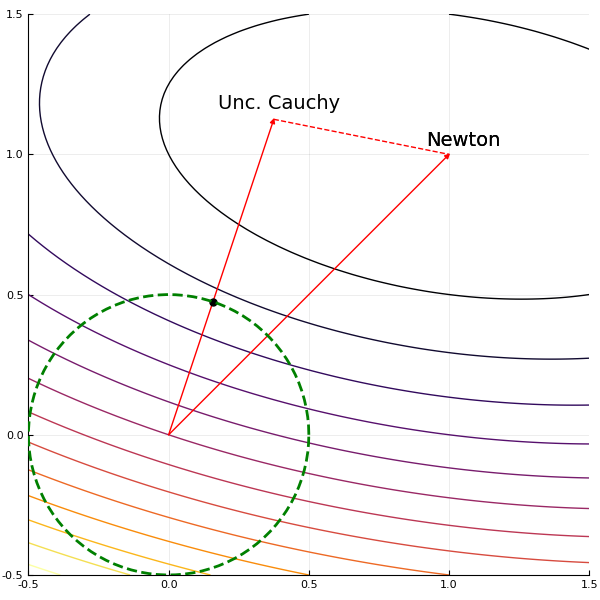
\includegraphics[width=0.3\textwidth]{src/krylov1.png}
  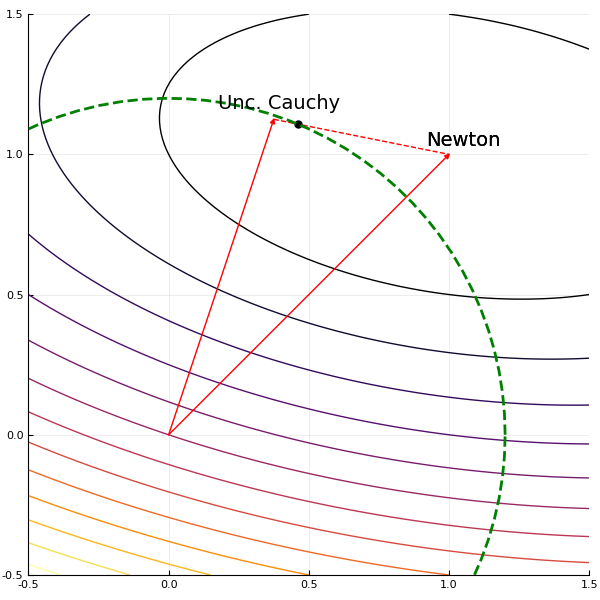
\includegraphics[width=0.3\textwidth]{src/krylov2.png}
  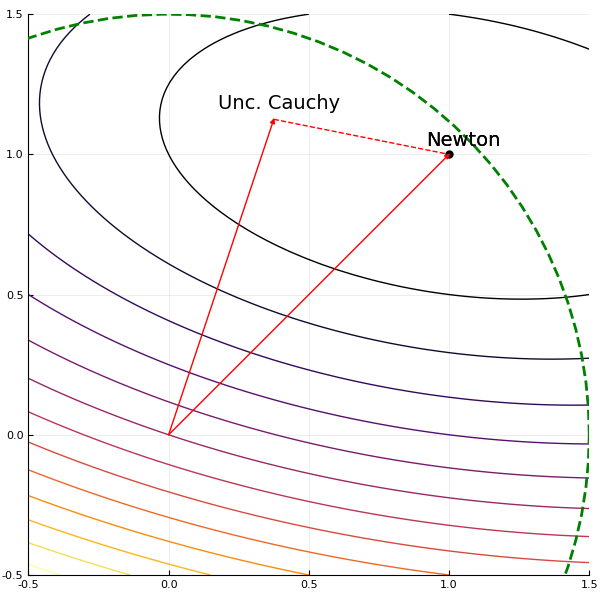
\includegraphics[width=0.3\textwidth]{src/krylov3.png}
\end{center}
\end{frame}

\begin{frame}[fragile,t]
  \ctr{Krylov + LBFGS}
\begin{lstlisting}
B = LBFGSOperator(n, scaling=false)
H = InverseLBFGSOperator(n, scaling=false)

s = rand(n)
y = rand(n)
push!(B, s, y)
push!(H, s, y)

v = ones(n)
cg(B, v)[1] - H * v
\end{lstlisting}
\end{frame}

\section{Optimize}

\begin{frame}[fragile,t]
  \ctr{Optimize}
  \begin{itemize}
    \item Tools for line search and trust region methods;
    \item Implementations of optimization methods, focusing on large-scale;
    \item Currently \verb+lbfgs+ and \verb+trunk+ for unconstrained problems,
      and \verb+tron+ for bound constrained problems.
    \item Tools for benchmarking (together with BenchmarkProfiles);
  \end{itemize}
\begin{lstlisting}
pnames = CUTEst.select(max_var=10_000, contype=:unc)
problems = (CUTEstModel(p) for p in pnames)
solvers = Dict{Symbol,Function}(:lbfgs => lbfgs, :trunk => trunk)
bmark_args = Dict(:max_f => 10_000, :max_time => 30.0)
stats, p = bmark_and_profile(solvers, problems, bmark_args=bmark_args)
png(p, "perfprof")
\end{lstlisting}
\end{frame}

\begin{frame}[fragile,t]
  \ctr{Optimize}
  \begin{center}
    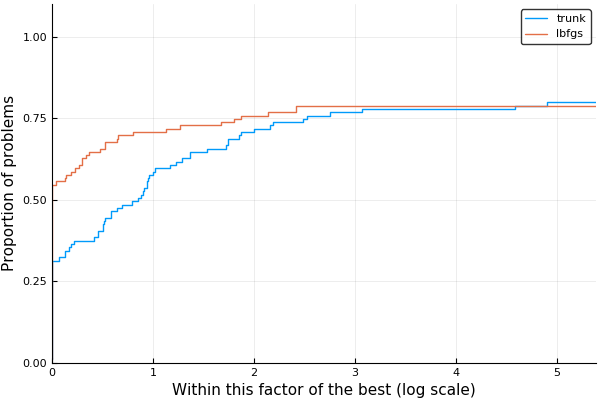
\includegraphics[height=0.75\textheight]{src/perfprof.png}
  \end{center}
\end{frame}

\begin{frame}[fragile,t,allowframebreaks]
\ctr{Optimize vs. Optim}
\begin{lstlisting}
function optim_method(nlp :: AbstractNLPModel; kwargs...)
  f(x) = obj(nlp, x)
  g!(storage, x) = grad!(nlp, x, storage)
  Dt = time()
  output = optimize(f, g!, nlp.meta.x0, LBFGS(m = 5),
                    Optim.Options(g_tol = 1e-8,
                                  iterations = 10_000_000,
                                  f_calls_limit = 10_000))
  Dt = time() - Dt
  status = output.g_converged ? :first_order : :unknown
  return GenericExecutionStats(status, nlp, solution=output.minimizer,
                               objective=output.minimum, dual_feas=output.g_residual,
                               iter=output.iterations, elapsed_time=Dt)
end
\end{lstlisting}
\end{frame}

\begin{frame}[fragile,t,allowframebreaks]
  \ctr{Optimize vs. Optim}
\begin{lstlisting}
solvers = Dict{Symbol,Function}(:Optim => optim_method, :Optimize => lbfgs)
pnames = sort(CUTEst.select(max_var=1000, contype=:unc))
bmark_args = Dict(:atol => 1e-8, rtol => 0.0, :max_f => 10_000, :max_time => 30.0)

problems = (CUTEstModel(p) for p in pnames)
stats, p = bmark_and_profile(solvers, problems)
png(p, "vs-optim-sum-counters")
stats, p = bmark_and_profile(solvers, problems, cost=stat->stat.elapsed_time)
png(p, "vs-optim-time")
\end{lstlisting}
\end{frame}

\myframe{
  \ctr{Optimize vs. Optim -
    \only<1>{Functions evaluations}\only<2>{Elapsed time},
    from 100 to 10000 variables
  }
  \begin{center}
    \only<1>{
      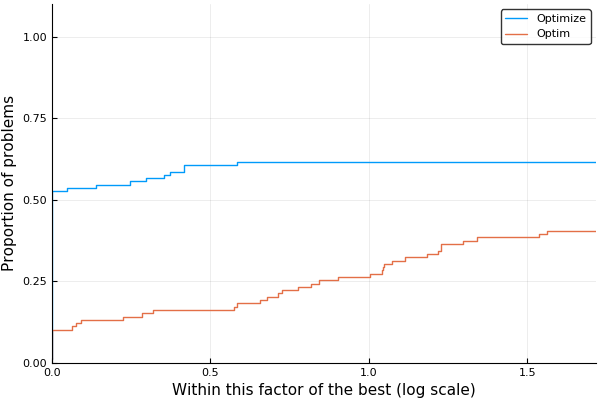
\includegraphics[height=0.75\textheight]{src/vs-optim-sum-counters-large.png}

    }
    \only<2>{
      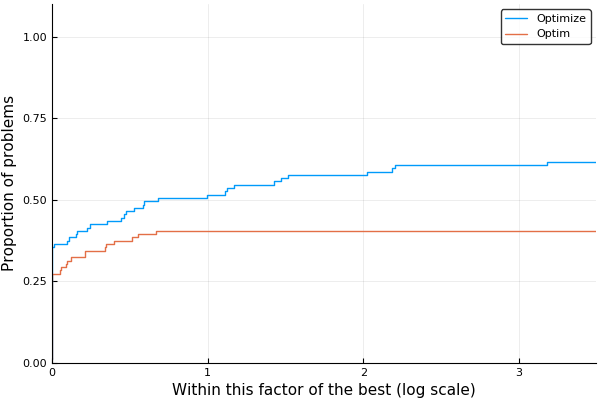
\includegraphics[height=0.75\textheight]{src/vs-optim-time-large.png}

    }
  \end{center}
}

\section{Remarks}

\myframe{
  \ctr{Summary}
  \begin{itemize}
    \item NLPModels for easy model creation and access;
    \item CUTEst + others for easy access to problems;
    \item LinearOperators + Krylov for factorization free methods;
    \item Optimize for benchmarking and subproblem solvers.
  \end{itemize}
}

\myframe{
  \ctr{Future Work}
  \begin{itemize}
    \item Code updates: Julia 0.7/1.0, MOI interface, and type stability;
    \item General constraints solver and stable version of Optimize;
    \item Parameter optimization;
    \item More problems natively in Julia, and problem classification;
    \item CUDA.
  \end{itemize}
}

\begin{frame}[allowframebreaks]
  \ctr{References}
  \printbibliography
\end{frame}
